\documentclass[12pt, a4paper, notitlepage, onecolumn]{article}

\usepackage[affil-it, blocks]{authblk}
\usepackage[margin=2cm]{geometry}
\usepackage[utf8]{inputenc}
\usepackage[russian]{babel}
\usepackage{setspace}


\usepackage{graphicx}
\usepackage{subcaption}
% \graphicspath{{pictures/}}
% \DeclareGraphicsExtensions{.eps,.pdf,.png,.jpeg}

\onehalfspacing
\renewcommand\Authand{ ~и~}
\renewcommand\Authands{ и }


% review
\usepackage[textwidth=120]{todonotes}
\usepackage{color}

% К статье в обязательном порядке прилагается экспертное заключение о возможности опубликования в открытой печати.
% Общий объем статьи вместе с рисунками, таблицами и литературой не должен превышать 4 (для приглашенного доклада — 5) страниц.
% Формат документа — LaTeX, стиль — article, 12 шрифт, полуторный интервал.
% В начале статьи указывается УДК (Универсальный Десятичный Классификатор). Статья должна предваряться аннотацией, ключевыми словами; обязательно указываются места работы (с адресами) авторов и электронный адрес докладчика. Рекомендуем использовать подготовленный шаблон.
% В конце статьи приводится её название, фамилии и места работы (аффиляции) авторов и основные термины на английском языке.
% Рисунки чёрно-белые, должны быть представлены в векторном формате, разрешение не ниже 600 DPI.
% Пожалуйста, загружайте в личный кабинет архив, содержащий скан экспертного заключения, исходные файлы (TeX-файл, рисунки) и скомпилированный pdf-файл.
% Список литературы оформляется в соответствии с приведёнными примерами: 



\begin{document}

\begin{flushright}
УДК {53.082.79}
\end{flushright}

\title{Проектирование детектора протонов и электронов для мониторинга солнечных космических лучей}
\author[1,2,3]{М. Зелёный%
  \thanks{Докладчик: mihail.zelenyy@phystech.edu}}
\author[1,2]{Е. Стадничук}
\author[1,2]{А. Нозик}
\author[3]{И. Зимовец}
\author[1]{А. Кудинов}
\author[1]{И. Резников}
\affil[1]{МФТИ (ГУ), 141701, Московская облаcть,
г. Долгопрудный, Институтский пер., 9.  \todo[author = Nozik, color = red]{Добавить полные адреса. Зелёный: Я посмотрел статьи, кто во что горазд, то и пишут в аффиляции}} 
\affil[2]{ИЯИ РАН, 117312, г. Москва, В-312, проспект 60-летия Октября, 7а.}%
\affil[3]{ИКИ РАН, 117997, г. Москва, ул. Профсоюзная 84/32}%

\date{}
{\let\newpage\relax\maketitle}

\begin{abstract}
В докладе представлен проект космического компактного \todo[author = Zimovets]{вместо "орбитального" лучше "космического компактного". Зелёный: заменил} детектора для измерения энергетических спектров протонов (10-100 МэВ) и электронов (до 10 МэВ) в солнечных космических лучах. Детектор может работать в двух режимах: дифференциальном (восстанавливается каждое событие) и интегральном (восстанавливается только энергетический спектр и состав излучения при большой загрузке).\todo[author = Nozik]{Поменял немного текст}
\end{abstract}

{\noindent \bf Ключевые слова:} детектор элементарных частиц, солнечные космические лучи, математическая статистика, анализ данных, компьютерное моделирование. 


\section*{Введение.} 
В результате спорадических \todo[author = Nozik]{Чего-то не нравится мне это слово. Зелёный: Это от Ивана. Зимовец: спорадический значит эпизодический, случайный. В нашей области этот термин часто используется.} явлений солнечной активности, таких как вспышки и корональные выбросов массы, электроны/ионы могут ускоряться до энергий в десятки МэВ/ГэВ соответственно, образуя так называемые  солнечные космические лучи (СКЛ)~\cite{miroshnichenko2015solar}. Несмотря на многолетнее интенсивное исследование СКЛ остается еще масса неразрешенных вопросов. До сих пор нет окончательного понимания механизмов ускорения частиц, их выхода из солнечной короны и распространения в межпланетной среде ~\cite{miroshnichenko2015solar}. Детальное понимание этих механизмов является фундаментальной задачей, поскольку схожие физические процессы происходят во многих астрофизических объектах. Более того, это требуется для построения надежного количественного прогноза СКЛ в различных точках гелиосферы, поскольку СКЛ могут оказывать серьезное негативное воздействие как на околоземные космические системы и межпланетные станции, так и на биологические объекты на их борту ~\cite{petrukovich2008cosmic}. Развитие космической техники и освоение космического пространства требует прогресса в изучении СКЛ и в идеале, создание разветвленной сети мониторинговых космических станций. Для этого, в частности, необходимо создание надежных, легких, компактных, потребляющих малую мощность детекторов энергичных частиц, способных одновременно измерять электроны и ионы в диапазонах энергий ~1-10 МэВ и ~10-100 МэВ соответственно. 

\section*{Описание детектора и методика измерения.}
В работе представлена концепция телескопа на основе сегментированного сцинтилляционного детектора. Методика измерения основана на анализе кривой зависимости ионизационных потерь (см. Рис.~\ref{pic-01-a} \todo[author = Nozik, color = red]{Увеличить толщину линий} ) от пробега частицы. По этой кривой можно с высокой точностью идентифицировать тип частицы и её кинетическую энергию, в том числе благодаря наличию у протонов характерной особенности - пика Брэгга в конце кривой ~\cite{Gruppen} \todo[author = Nozik, color = red]{Ссылку! Зелёный: сослался на Группена}.
\begin{figure}[ht!]
	\begin{subfigure}[b]{0.5\textwidth}
    	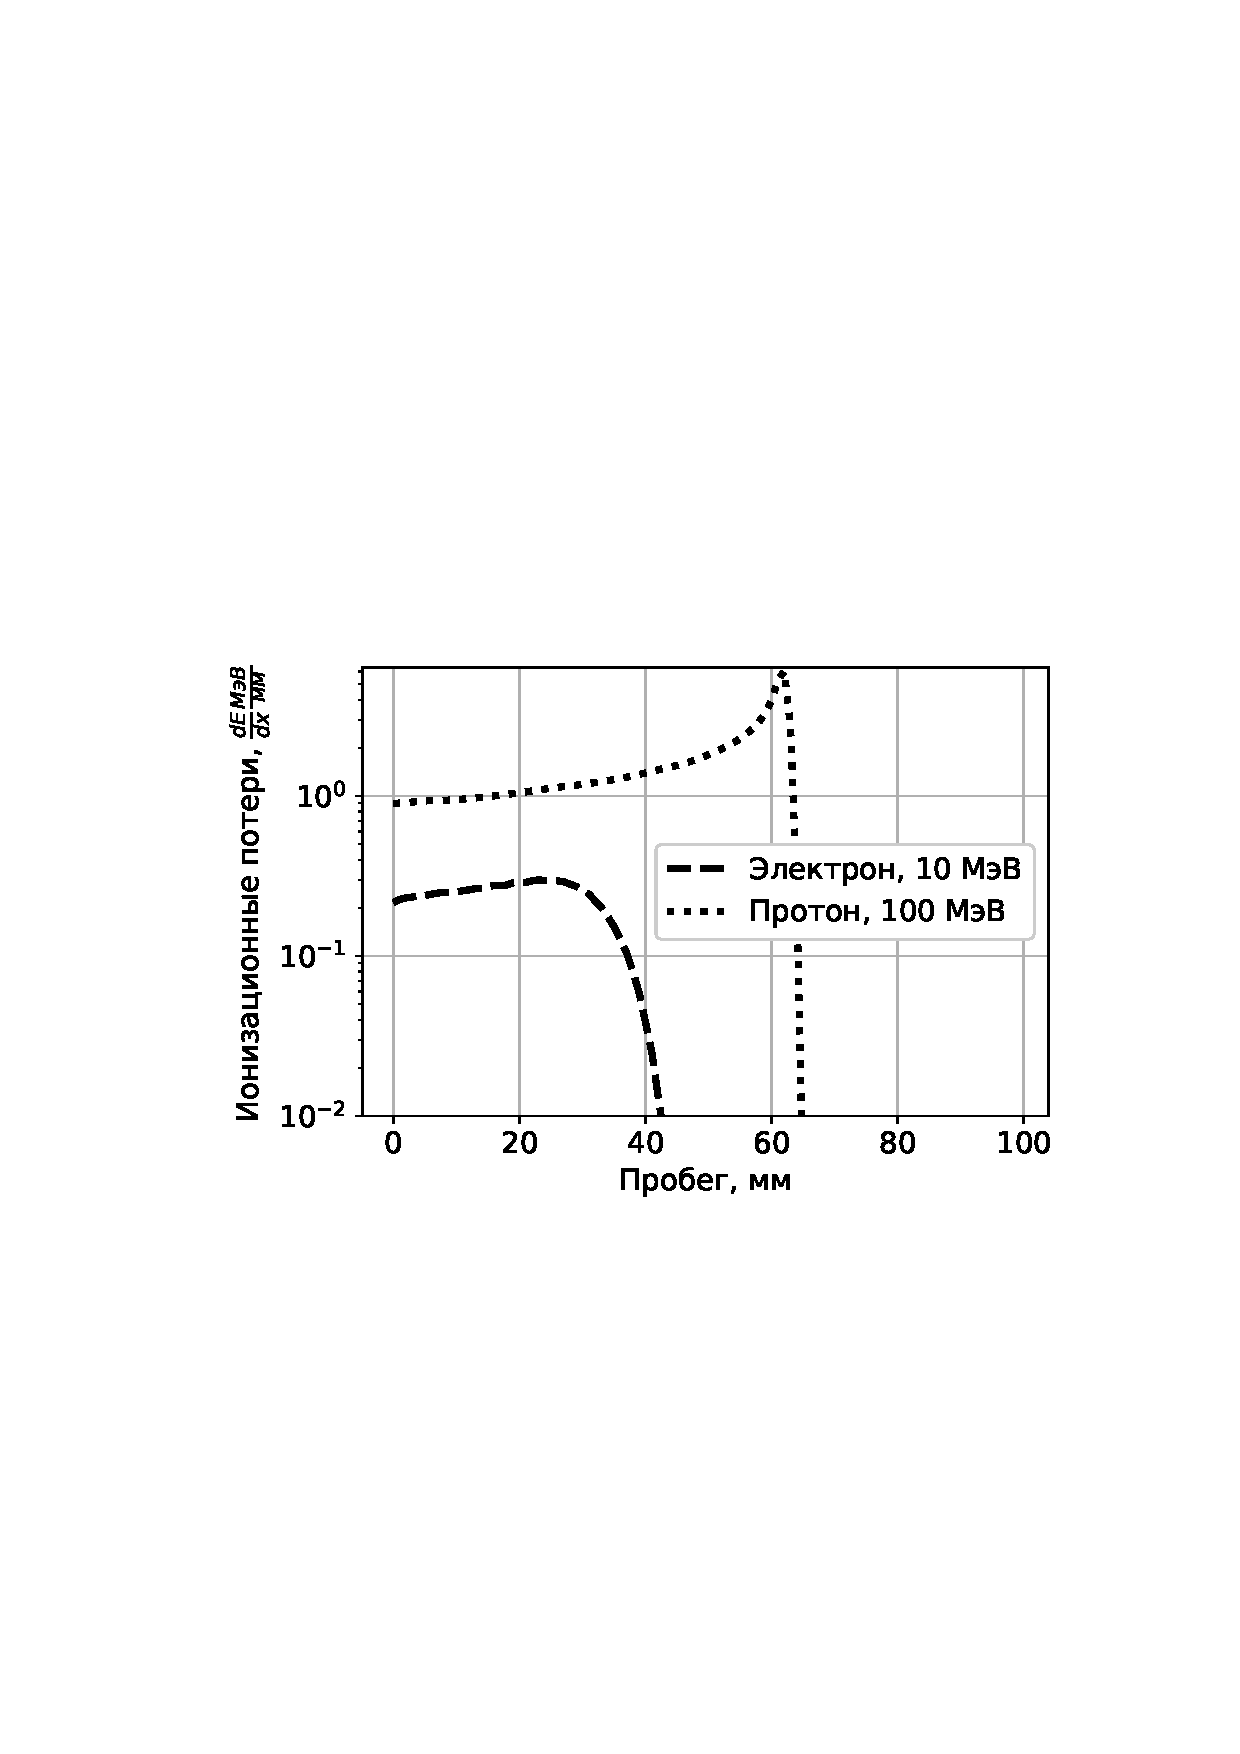
\includegraphics[width=0.95\linewidth]{pictures/01_bregg.pdf}
        \caption{}
        \label{pic-01-a}
    \end{subfigure}
	~
    \begin{subfigure}[b]{0.5\textwidth}
		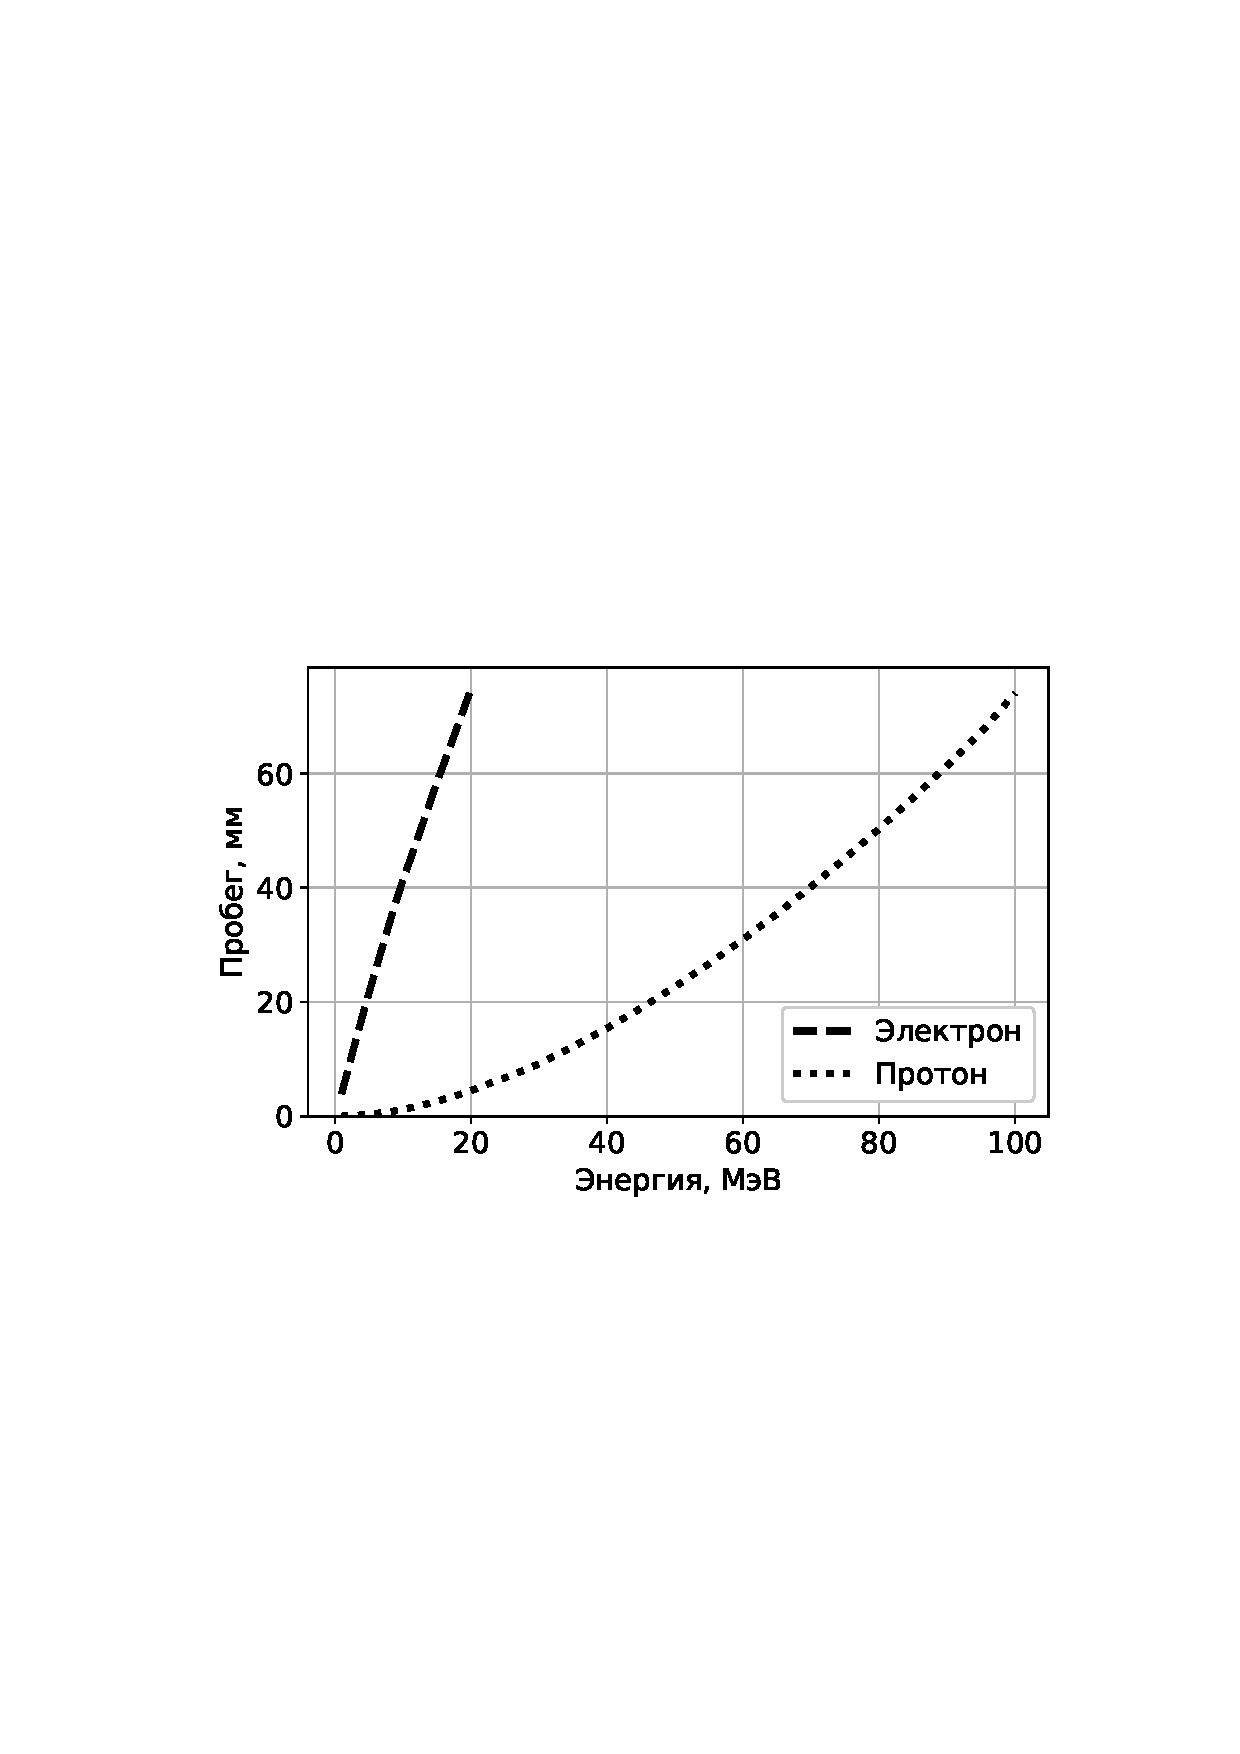
\includegraphics[width=0.95\textwidth]{pictures/02_range.pdf}
        \caption{}
        \label{pic-01-b}
    \end{subfigure}
    \caption{ a) Зависимость выделенной энергии от глубины для электрона и протона в антрацене. b) Полная длина пробега для протонов и электронов в антрацене}
\end{figure}
Телескоп представляет собой набор цилиндрических сцинтилляционных шайб, диаметром 2-5 см, разделенных светоотражающим материалом, помещенных в металлический корпус. В одном или нескольких местах в шайбе делается скос или “ушко” для установки фотоумножителя. Для обеспечения равномерного светосбора рассматриваются варианты с установкой до трех фотоумножителей на одну шайбу или с кольцевым оптоволокном. Места установки детекторов в последовательных шайбах могут быть сдвинуты друг относительно друга на $60^\circ$ для того, чтобы слои можно было делать достаточно тонкими и детекторы в соседних слоях не мешали друг другу. Входное окно телескопа остается открытым, но при необходимости на него может быть установлен коллиматор или фильтр низкоэнергетичных частиц (например, бериллиевое покрытие может отфильтровывать низкоэнергетичные протоны, при этом являясь прозрачным для электронов в  интересующем нас диапазоне энергий, из Рис.~\ref{pic-02-a} следует что оптимальным будет использовать напыление с толщиной 400-500 мкм). Толщина шайб может быть выбрана разной в зависимости от конкретных задач детектора (более тонкие слои позволяют получить лучшее разрешение, но при этом увеличивается вес детекторов и сопутствующей электроники). В общем случае предполагается, что вблизи входного окна плотность слоев выше, поскольку там требуется большая точность определения формы кривой потерь (для идентификации электронов). Минимальная толщина может составлять от 2 мм. Вдали от входного окна толщина увеличивается и достигает 5-10 мм. Полная толщина детектора может варьироваться в зависимости от необходимости снизить массу детектора или расширить диапазон регистрируемых энергий, так из Рис.~\ref{pic-01-b} следует, что для полного поглощения протонов с энергией 100 МэВ требуется 65 мм антрацена. Корпус прибора частично обеспечивает пассивную защиту от боковых частиц (см. Рис.~\ref{pic-02-b}), поглощая протоны с энергией 20-40 МэВ и электроны до 4 МэВ.
\begin{figure}[ht!]
	\begin{subfigure}[b]{0.5\textwidth}
    	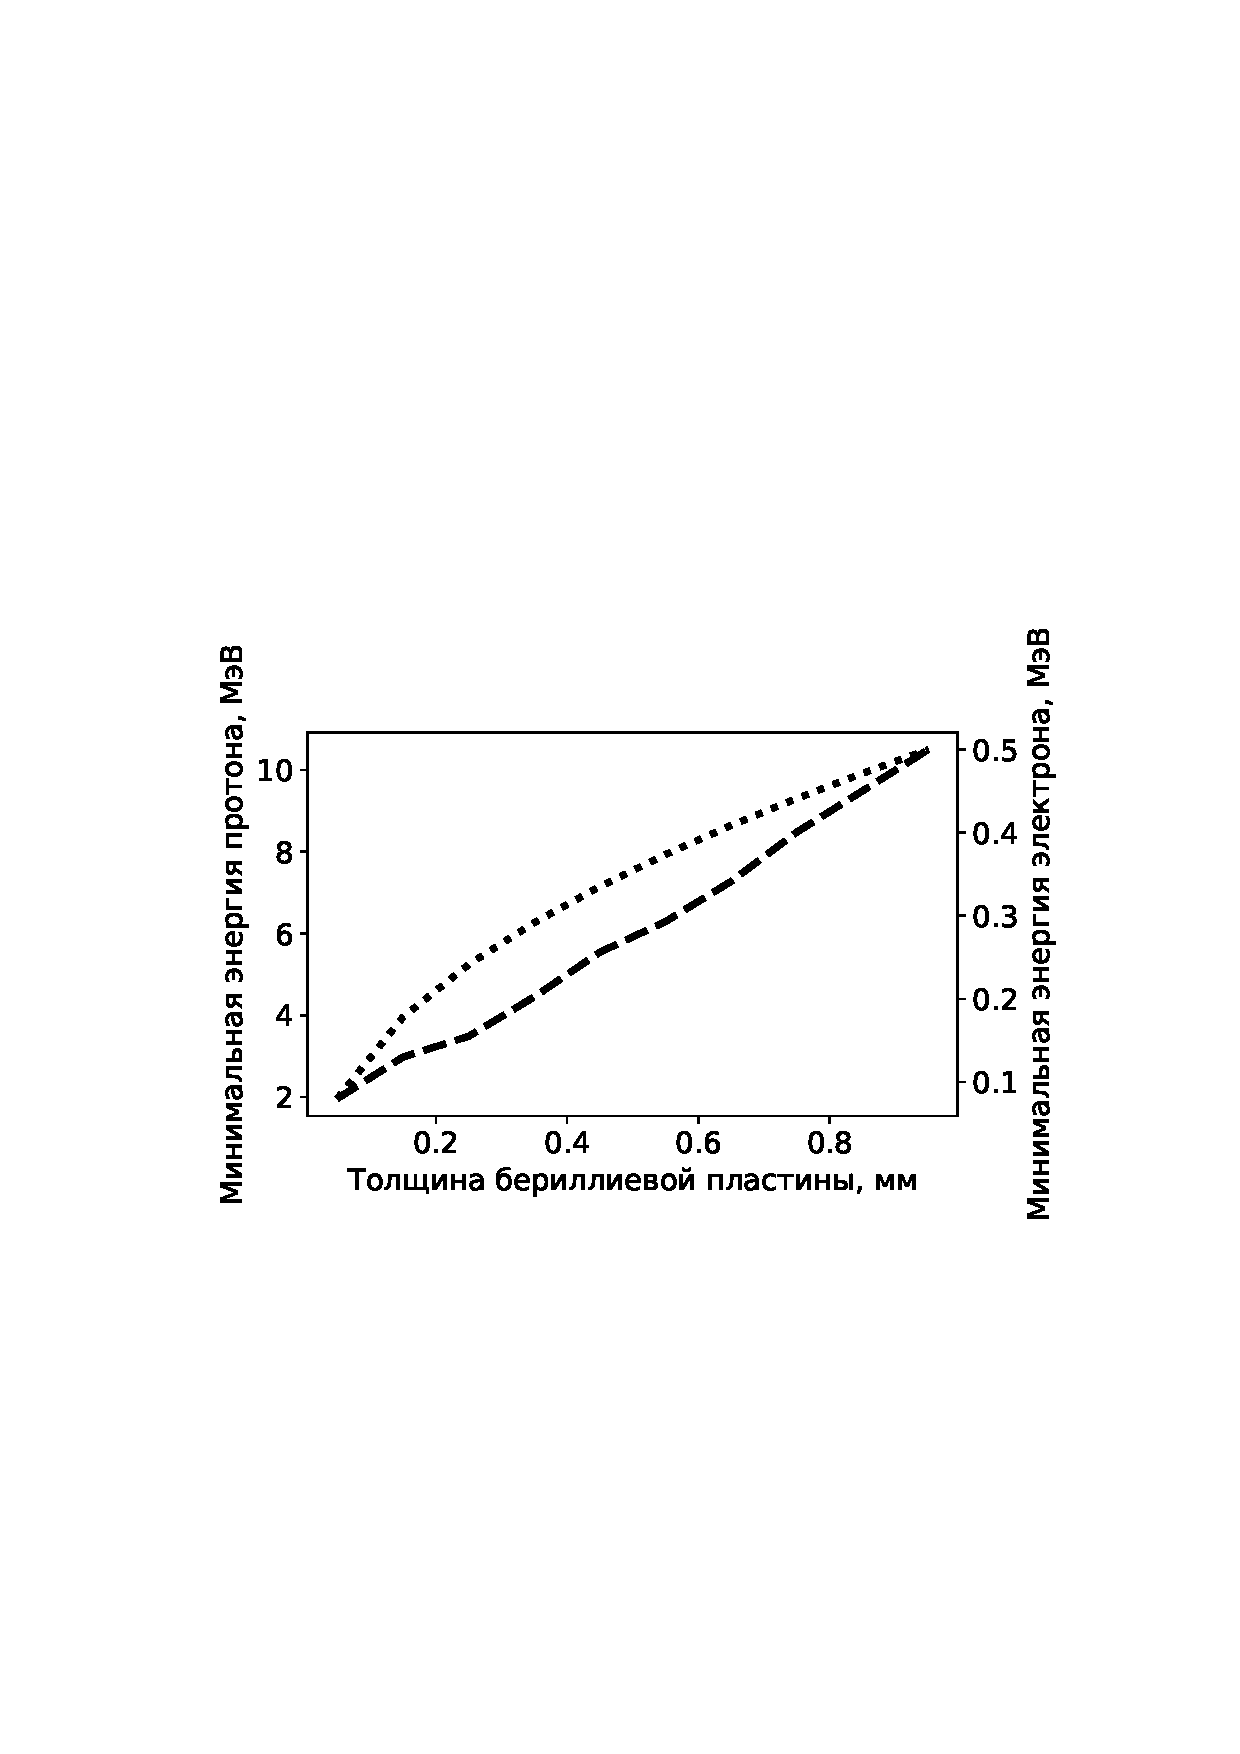
\includegraphics[width=0.95\linewidth]{pictures/03_berillium.pdf}
        \caption{}
        \label{pic-02-a}
    \end{subfigure}
	~
    \begin{subfigure}[b]{0.5\textwidth}
		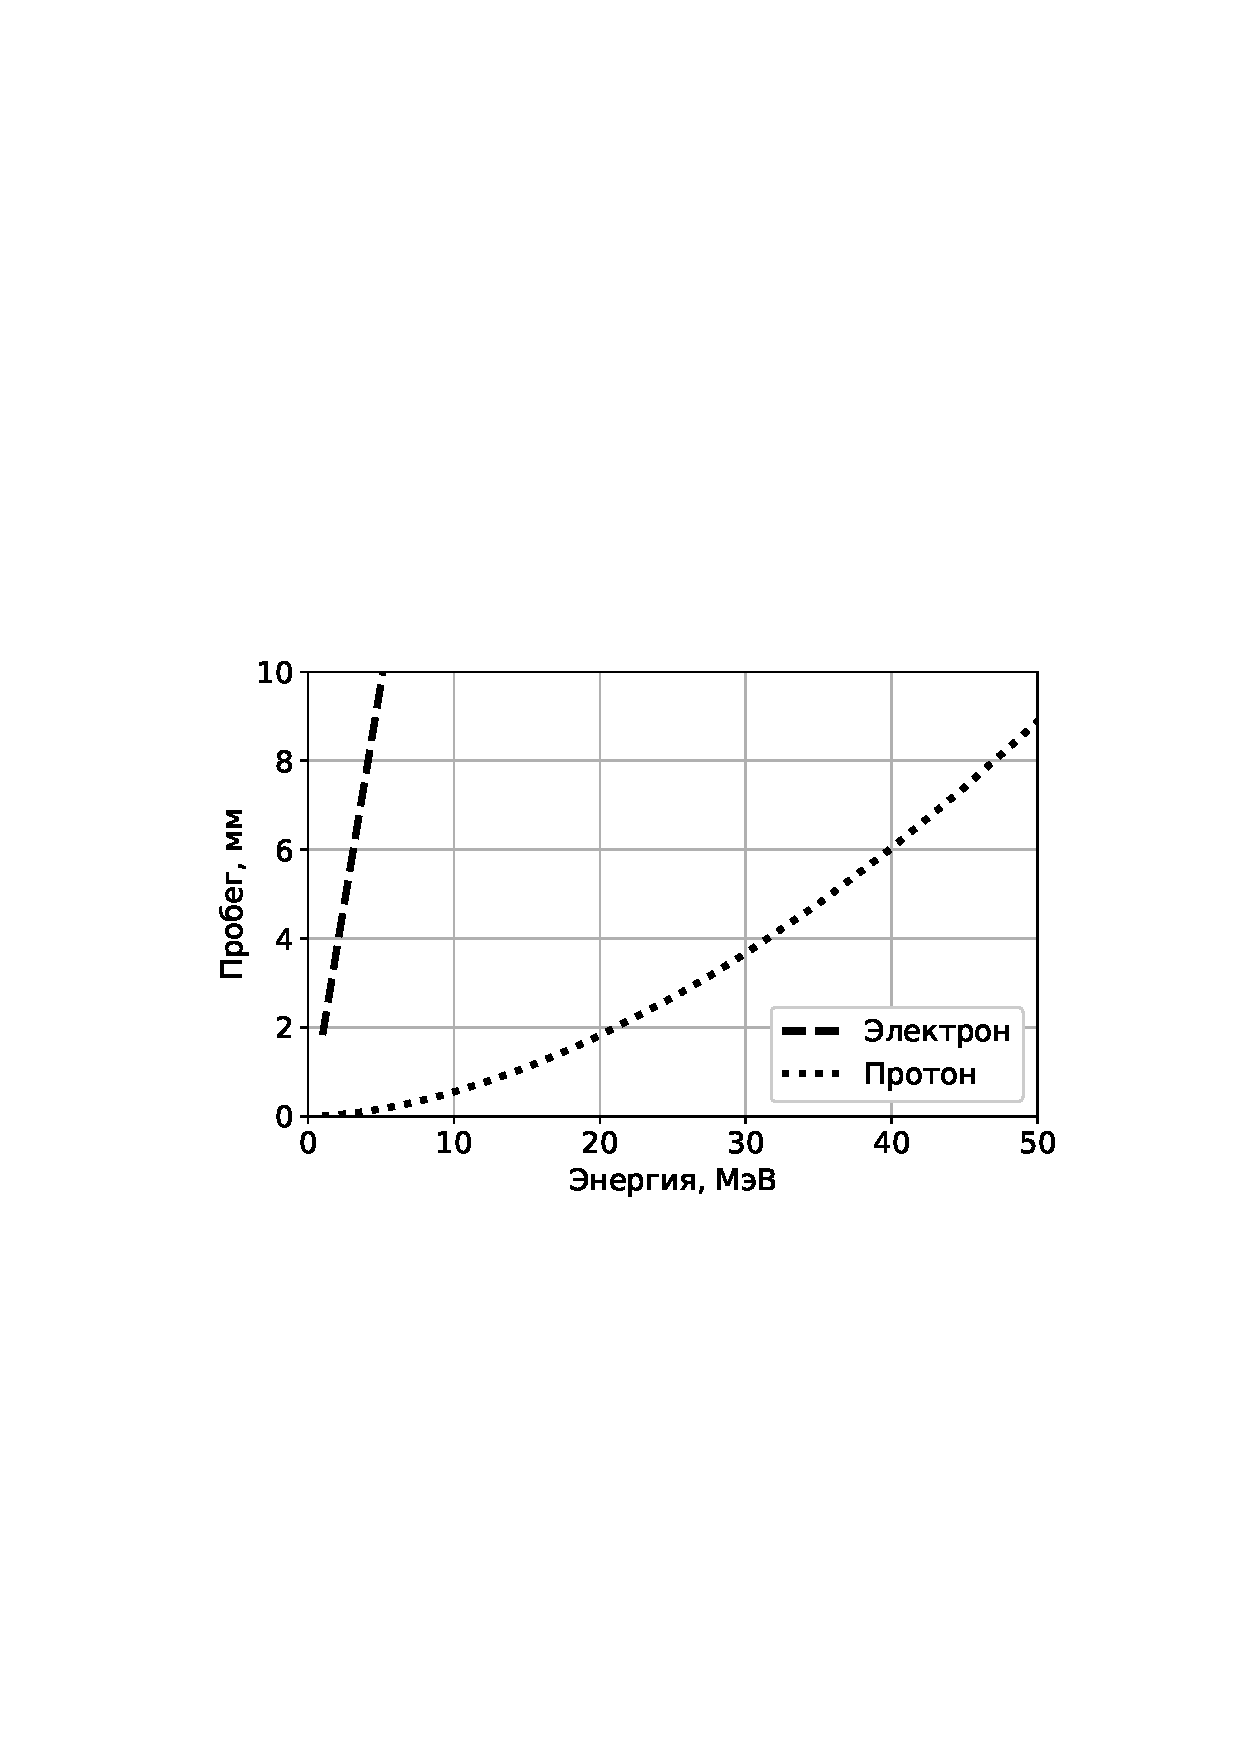
\includegraphics[width=0.95\textwidth]{pictures/04_casing.pdf}
        \caption{}
        \label{pic-02-b}
    \end{subfigure}
    \caption{ a) Бериллий. b) Полная длина пробега для протонов и электронов в D16}
\end{figure}

\section*{Моделирование и методика анализа.}
Из-за нестабильности величины потока солнечных частиц для детектора предусмотрены 3 режима работы: при низкой скорости счета производится анализ каждого события, а при превышении некоторого порога (обусловленного скоростью работы электроники и временем высвечивания сцинтиллятора) идет накопление суммарного сигнала за некоторый промежуток времени, а затем восстанавливается энергетический спектр частиц, попавших в детектор за это время. Третий режим является смешанным: в шайбах, расположенных вблизи входного окна, проводится измерение суммарных ионизационных потерь, а в дальних шайбах производится идентификация отдельных событий. В качестве основы для анализа используются рассчитанные значения ионизационных потерь и набор триггеров для отсечения событий. Для расчета энерговыделения в сцинтилляционных шайбах проведено Монте-Карло моделирование при помощи транспортного кода GEANT4 ~\cite{ALLISON2016186}.  В качестве физической модели использовался модуль стандартной электромагнитной физики GeEmStandartPhysics, включающий в себя описание процессов, оказывающих основное влияние на распространение частиц в детекторе: ионизационные потери и их флуктуации, упругое кулоновское рассеяние и тормозное излучение электронов.

В одночастичном режиме для анализа отбираются события, прошедшие через входное окно, и, исходя из полной измеренной энергии и количества сработавших слоев, определяются диапазоны возможных параметров частицы, а также отсекаются события, пришедшие под большими углами. В данных диапазонах параметров определяется набор параметров, максимизирующий значение функции правдоподобия --- произведения вероятностей наблюдать измеренное энерговыделение при данном наборе параметров. Предварительный алгоритм позволяет определить энергию протонов с точностью 1 МэВ для исходной энергии 50 МэВ, то есть дает точность порядка 2\%.

Для анализа спектра в интегральном режиме разрабатывается процедура, основанная на методике регуляризации обратных задач, разработанной В. Ф. Турчиным ~\cite{Turchin-epf}. 

% Мы представляем дифференциальный спектр в виде разложения: 
% \begin{equation}
% \label{diffSpectrum}
% \varphi(E) = \sum \limits_{n} \varphi_n T_n(E),
% \end{equation}
% где $E$ - энергия частицы, $T_n(x)$ - полиномы Берштейна~\cite{korovkin2001bernstein}. Пусть $K_j(E)$ --- потери энергии частицы с энергией $E$ в j-ом сегменте детектора (На ~\ref{pic-03-a} приведена функция $K_j(E)$ для одного из сегментов детектора, рассчитанная на основе моделирования). Тогда полное энерговыделение $f_j$ в j-ом сегменте связано с дифференциальным спектром по формуле:
% \begin{equation}
% \label{intSpectrum}
% f_j = \int K_j(E) \varphi(E)~dE
% \end{equation}
% Подстановка разложения ~\ref{diffSpectrum} в ~\ref{intSpectrum} даёт систему линейных уравнений:
% \begin{equation}
% f_j = \sum \limits_{n} \varphi_n \int K_j(E) T_n(E)~dE  = \sum \limits_{n} \varphi_n C_{nj},
% \end{equation}
% которая может быть решена согласно ~\cite{Turchin-epf}. 

Предварительный (не оптимизированный ) результат применения процедуры для восстановления данных, симулирующих лобовой пучок протонов в детекторе из 20 сегментов (10 сегментов по 2 мм, 5 по 3 мм и 5 по 5 мм), приведен на Рис.~\ref{pic-03-b}, пример референтной кривой поглощения в одном сегменте детектора,используемой для восстановления спектра, приведен на Рис.~\ref{pic-03-a}. % Добавил пояснение к картинке 3a

\begin{figure}[ht!]
	\begin{subfigure}[b]{0.5\textwidth}
    	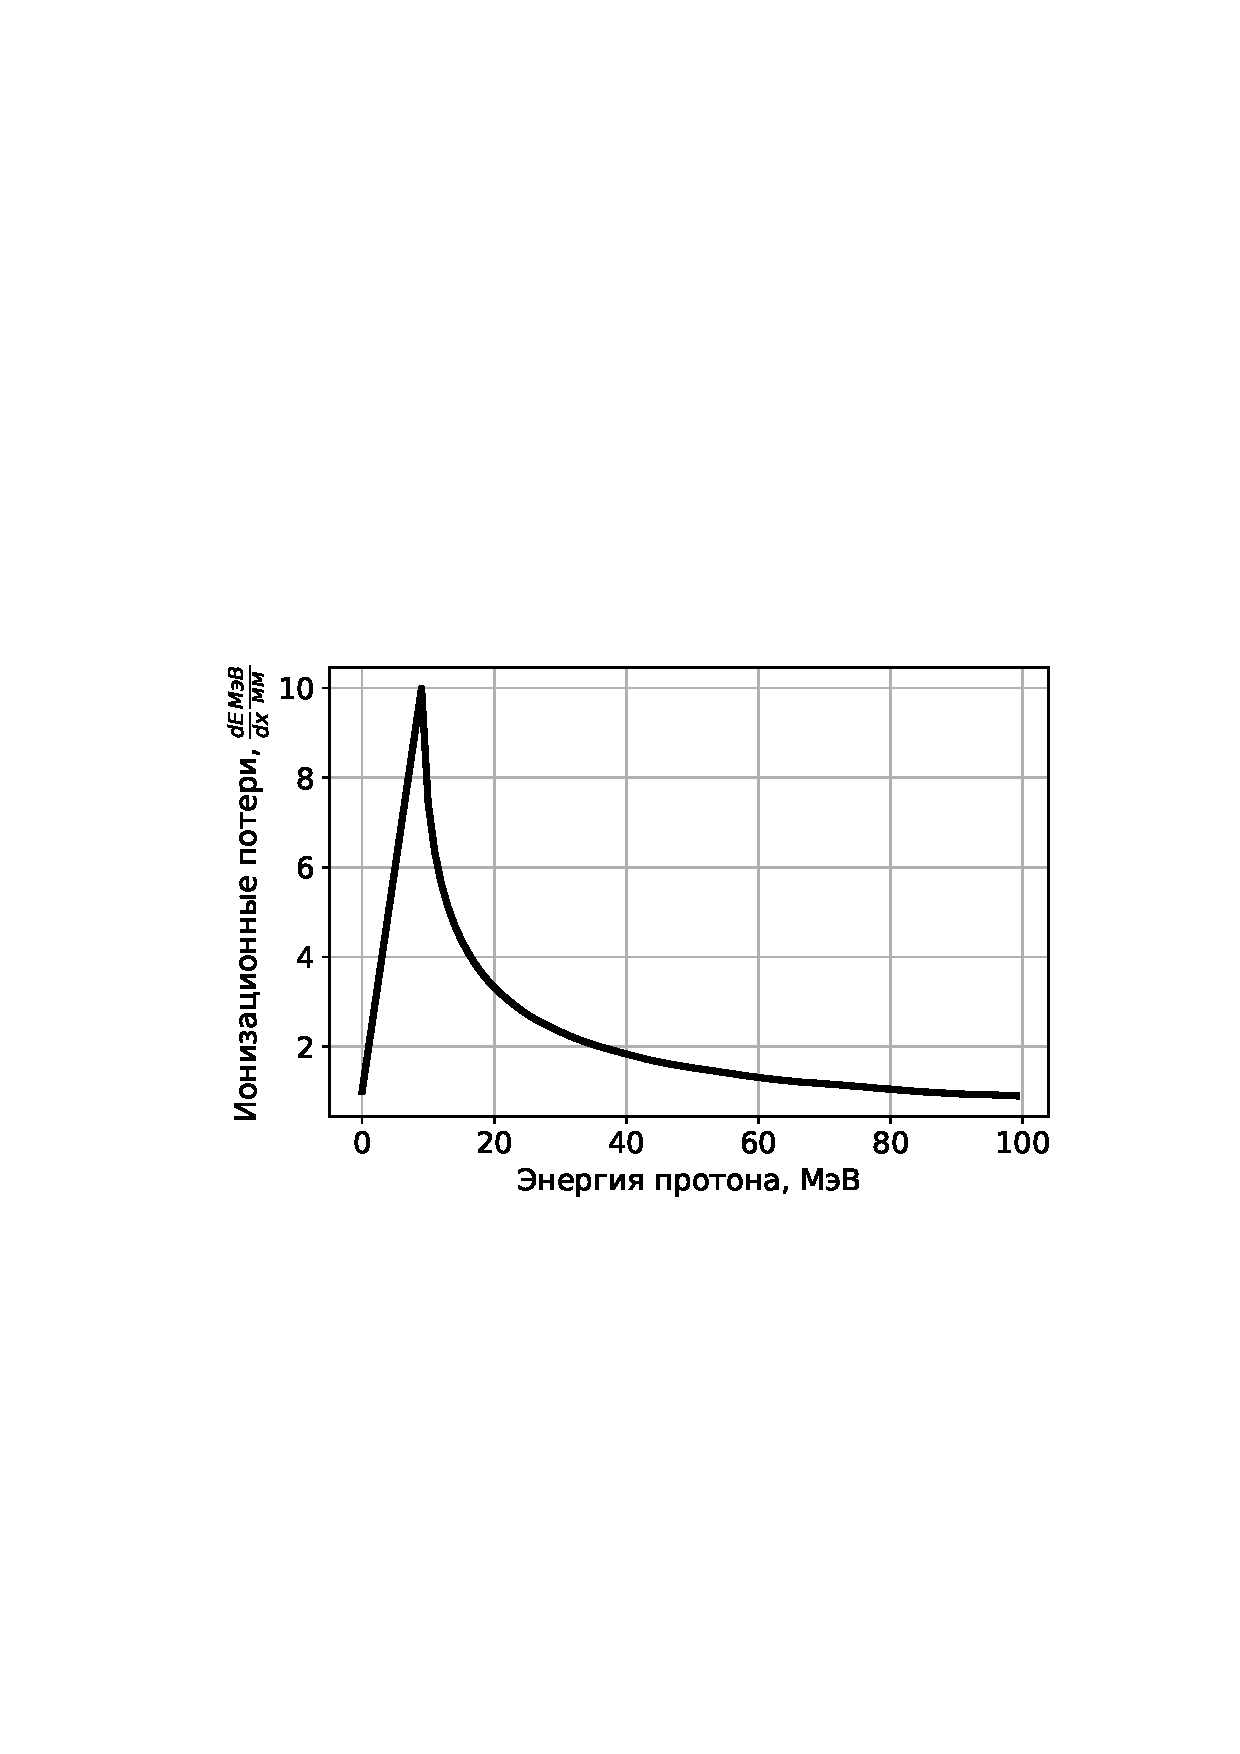
\includegraphics[width=0.95\linewidth]{pictures/05_LossInCell.pdf}
        \caption{}
        \label{pic-03-a}
    \end{subfigure}
	~
    \begin{subfigure}[b]{0.5\textwidth}
		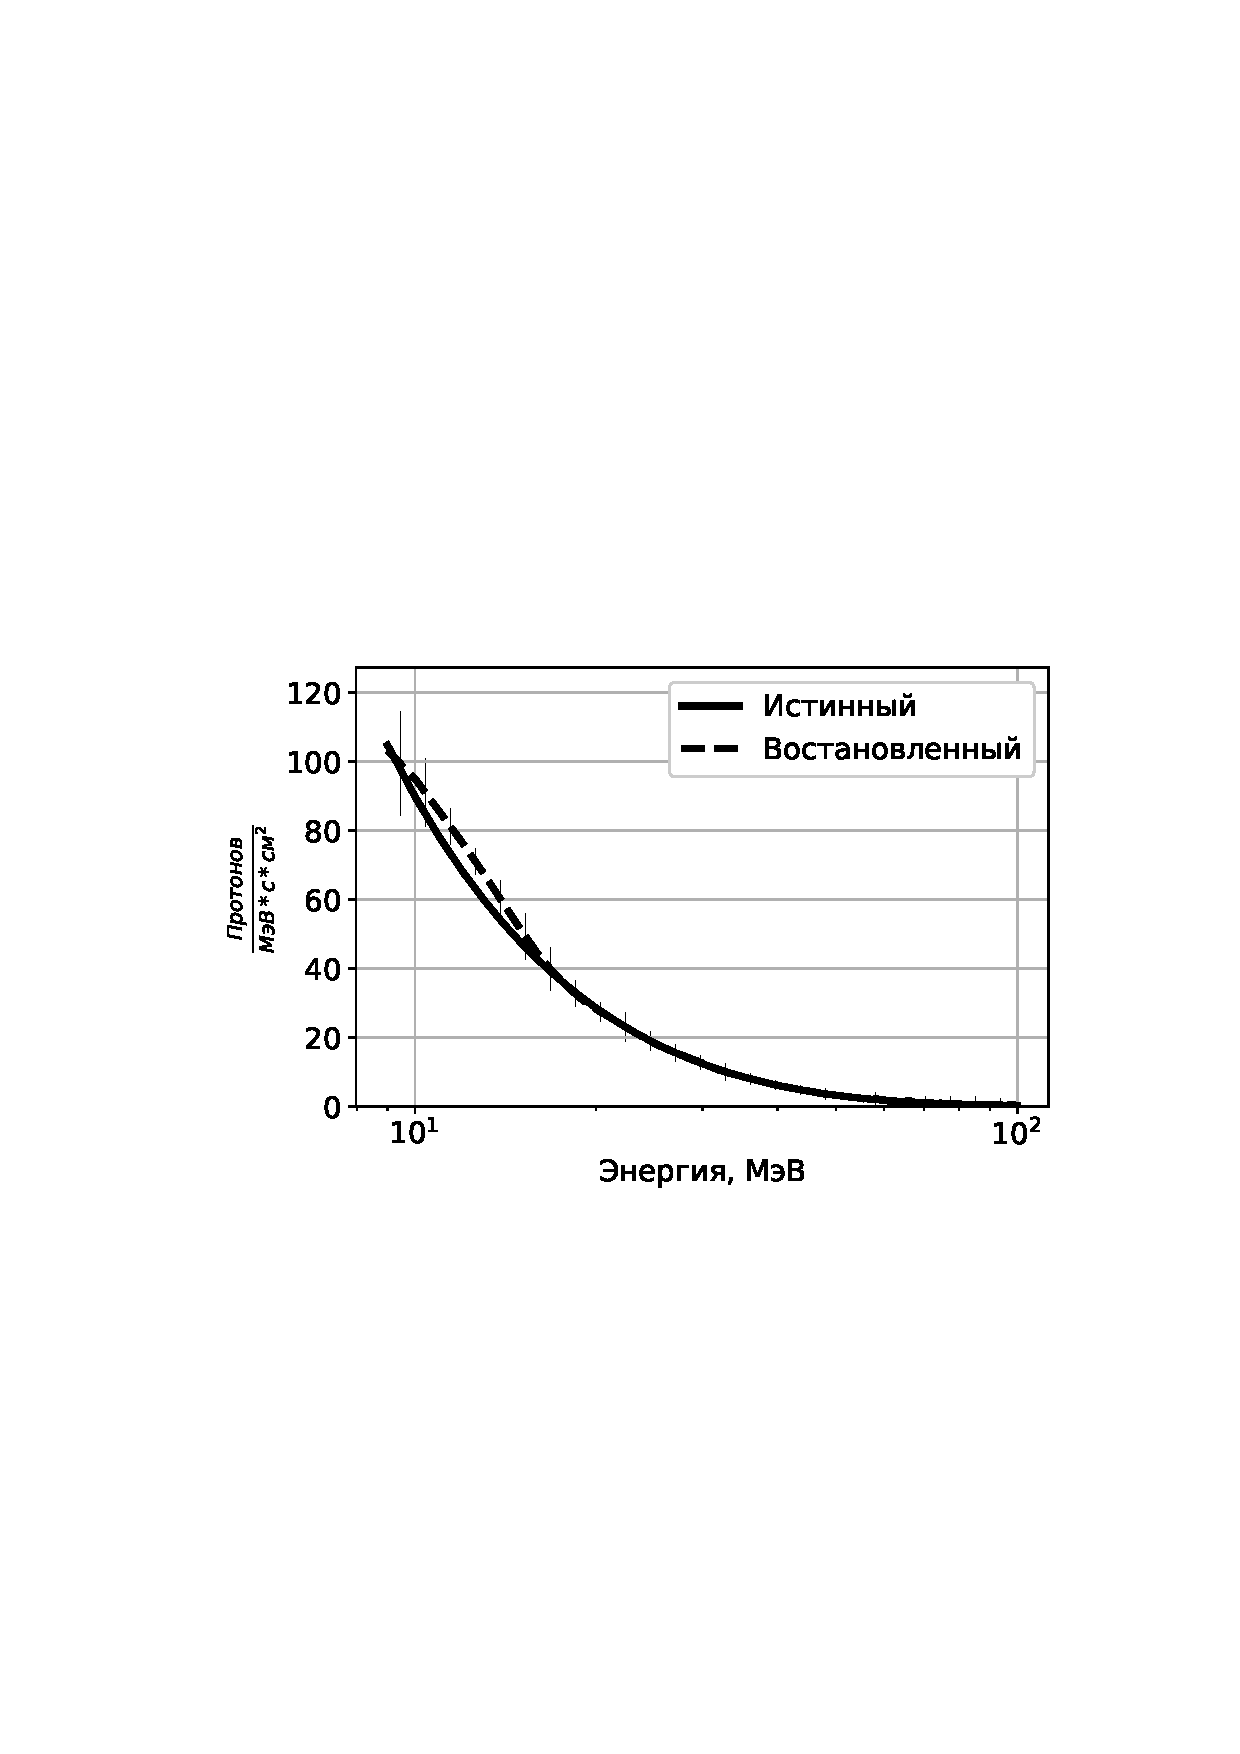
\includegraphics[width=0.95\textwidth]{pictures/06_IntegralSpectrum.pdf}
% * <ivanzimovets@gmail.com> 2018-05-18T06:16:14.968Z:
% 
% (b) Восстановленный
% 
% ^.
        \caption{}
        \label{pic-03-b}
    \end{subfigure}
    \caption{ a) Зависимость выделенной энергии от начальной энергии частицы в первом сегменте детектора. b) Результат восстановления дифференциального спектра.}
\end{figure}

% Метод наименьших квадратов может быть кратко описан следующим образом. Необходимо восстановить энергетический спектр частиц, попавших в детектор, по их суммарной кривой потерь. Спектр частиц ищется в виде разложения по полиномам Берштейна:
% \begin{equation}
% \varphi(E) = \sum \limits_{n} \varphi_n T_n(E)
% \end{equation}


% Следовательно, задача о восстановлении спектра частиц свелась к решению переопределённой системы линейных уравнений. Такие системы решаются, например, с помощью метода наименьших квадратов:
% \begin{equation}
% \vec{\varphi} = (C^T C)^{-1} C^T \vec{f}
% \end{equation}

\section*{Результаты.}
Разработана концепция секционного сцинтилляционного телескопа для регистрации энергичных электронов и протонов солнечного происхождения. Произведены работы по моделированию детектора и сделаны оценки его чувствительности для различных частиц и в различных диапазонах энергий. Предварительные результаты показывают, что при весе до 1 кг, детектор сможет позволить измерение энергетического спектра протонов от 5 до 100 МэВ и электронов от 1 до 10 МэВ с точностью порядка 1-5\%.

Существенным преимуществом детектора является возможность работы в так называемом интегральном режиме, когда не регистрируются индивидуальные частицы, а идет анализ полного пространственного спектра потерь энергии. Интегральный режим позволяет работать при скоростях счета более 1 МГц, обеспечивая при этом достаточно хорошую (около 5\%) точность восстановления исходного спектра и состава излучения.

\section*{Благодарности.}
Исследование выполнено за счет гранта Российского научного фонда (проект № 17-72-20134).

\bibliographystyle{unsrt}
\bibliography{references}
% * <ivanzimovets@gmail.com> 2018-05-18T06:29:51.467Z:
% 
% Некорректно дана ссылка [2] Петрукович и др. Это не отдельная книга, а глава в  томе II монографии  "Плазменная гелиогеофизика" (см., например, http://fireras.su/biblio/wp-content/uploads/51219.pdf) 
% 
% ^.


% Методы и материалы


% В данной работе была поставлена задача максимизировать разрешение детектора в интересующем энергетическом диапазоне и при этом минимизировать его массу, чтобы его можно было использовать в космосе. В первую очередь была оптимизирована геометрия детектора. На рисунке 3 представлены пробеги протонов и электронов в антрацене в зависимости от их кинетической энергии. Из этих графиков следует, что для того, чтобы регистрировать интересующие частицы, длина детектора должна составлять порядка 7 сантиметров.

% Список терминов, сокращений и перевод
% Спорадические явления – sporadic phenomena
% Солнечная активность – solar activity
% Солнечная вспышка – solar flare
% Солнечные космические лучи (СКЛ) – solar cosmic rays (SCR)
% Галактические космические лучи (ГКЛ) – galactic cosmic rays (GCR)
% События наземных возрастаний (СНВ) – ground level events (GLE)
% Корональный выброс массы (КВМ) – coronal mass ejection (CME)
% Космический аппарат (КА) – spacecraft 
% Полупроводниковый детектор (ППД) – solid state detector (SSD)
% Фотоэлектронный умножитель (ФЭУ) – Photomultiplier (PMT) 
% Гелиосфера – Heliosphere
% Гелиодолгота - Heliolongitude
%%Конец введение от Ивана


% В связи с освоением космоса растёт потребность в космических приборах. Одним из таких приборов является детектор элементарных частиц. Детекторы используются в различных целях. Во-первых, научный интерес представляет исследование солнечного ветра. Во-вторых, необходима система прогнозирования космической погоды. Такая система позволяет предупреждать космические станции о радиационной опасности, что способствует заблаговременному принятию мер по защите космотавтов и электроники. Например, разрабатывается методика предсказания потока протонов солнечного ветра по зарегистрированному потоку солнечных электронов. Таким образом, существует острая необходимость в разработке детекторов частиц для космических аппаратов.

% Целью настоящей работы является создание общей схемы детектора для измерения энергетического спектра частиц в космосе, а также разработка методики для оптимизации параметров детектора под различные задачи. Детектор представляет собой цилиндр, состоящий из множества тонких слоёв сцинтиллятора. Слои сцинтиллятора имеют разную толщину. На входе в детектор они тонкие, что увеличивает разрешение прибора при регистрации частиц низкой энергии. Далее их толщина постепенно увеличивается, что немного ухудшает разрешение прибора, но упрощает процесс изготовления и уменьшает число каналов для электроники. Спектр восстанавливается по потерям энергии частиц в каждом слое сцинтиллятора. Детектор работает в двух режимах: интегральный и счётный. При небольших потоках частиц скорость электроники позволяет идентифицировать каждую частицу отдельно по её кривой потерь. В таком случае детектор работает в счётном режиме. Когда поток частиц превышает скорость считывания электроники, например, при солнечных вспышках, детектор переходит в интегральный режим, а спектр частиц восстанавливается по интегральной кривой потерь. Для анализа данных в интегральном режиме используется метод регуляризации Турчина. Подробно методика восстановления спектра описана в разделе методология.

% В первую очередь прототип детектора разрабатывается для измерения быстрых солнечных частиц. Поэтому прибор нацелен на регистрацию протонов и электронов с кинетической энергией в диапазоне от 10 до 100 МэВ и от 0.1 до 10 МэВ соответственно. При этом детектор должен быть лёгким и компактным, чтобы его можно было использовать в космосе. В связи с этим были подобраны оптимальные параметры для цилиндра из сцинтиллятора. Во-первых, в качестве материала был выбран антрацен???. Во-вторых, длина цилиндра составляет 5 см???.  Наконец, радиус детектора был выбран ????. Также для подавления шумов от протонов и электронов, чья энергия ниже интересующего энергетического диапазона, на лицевую сторону детектора установлено бериллиевое окно. Оно поглощает протоны и электроны с кинетической энергией меньше 10 МэВ и ??? соответственно. При этом кривая потерь для частиц с большей энергией практически не искажается. Такие характеристики позволяют создать лёгкий детектор с хорошим разрешением.  Подробнее анализ параметров детектора приведён в разделе методология. Демонстрация работы компьютерной модели детектора и его предполагаемая разрешающая способность приведены в разделе результаты.

% Разработанная методика позволяет настраивать данный детектор под различные задачи. Установка, частью которой будет являться этот детектор, может быть использована для анализа космической погоды не только на околоземной орбите, но также может быть сконфигурирована для измерений в межпланетном пространстве, на лунных и марсианских базах.
\end{document}
